\chapter{Background and Related Work\label{cha:chapter2}}
dkjekdede dejfekjfhkjehf jefkjefkjefkje jekfnkejfbkjebfkje kejfbnekjfbjkebfekjfnekjfbnkjebf kjenfk jbkejfkjenfkj nejk kjn kj kjbjkbkjbkjb kj bkj jk bkjb kjb kj bkj bkj bkj bkjb kj  kjbkjbkjbkjbkj
kjhkjhkjhjk kjhkjhjkh kjhkjhkjh kjhkjhk kjhjkhkj.

\section{Context-awareness\label{sec:back_con_aw}}
In this section, the terms "context" and ''context-aware computing'' are discussed in more detail. Furthermore, application possibilities of context awareness is demonstrated.

In order for computers to assist users in their everyday tasks, they should adapt themselves to the current user's situation, and then respond according to this situation. 

Humans are quite successful at conveying ideas to each other and reacting appropriately. This is due to many factors: the richness of the language they use, the common understanding of how the world works, and an implicit understanding of every-day situations. When humans talk with each other, they are able to use implicit situational information, or \emph{context}, to increase the conversational bandwidth. Unfortunately, this ability to convey ideas does not transfer well to humans interacting with computers.\citeauthor{Dey2000b}

\subsection{What is Context?}

The report that first introduces the term \emph{context-aware}, [\citeauthor{ieee313011}] refers to context as location, identities of people and objects nearby, and changes to those objects. A similar definition, [\citeauthor{ieee626984}] describes context as location, identities of the people around the user, the time of day, season, temperature, etc. [\citeauthor{Ryan97}] defines context as the user's location, environment, identity and time. [\citeauthor{Dey98}] enumerates context as the user's emotional state, focus of attention, location and orientation, date and time, objects, and people in the user's environment. %These definitions that define context by certain examples are difficult to apply. In order to determine whether certain types of information not listed in the definition are correct context or not, it is difficult to determine how we can use the definition to solve this dilemma.

A recent definition of context-awareness is described by [\citeauthor{Dey2000b}] who defines it as, Context is any information that can be used to characterize the situation of an entity. An entity is a person, place, or object that is considered relevant to the interaction between a user and an application, including the user and applications themselves. 

This way it is easier for an application developer to enumerate the context for a given application scenario. If a piece of information can be used to characterize the situation of a participant in an interaction, then that information is regarded as context.

After the term ''context'' has been defined the term ''context-aware computing'' is discussed in the following subsection.

\subsection{Context-aware Computing}
Context-aware computing was first described by [\citeauthor{ieee313011}] in 1994 to be software, that adapts according to its location of use, the collection of nearby people and objects, as well as changes to those objects over time. However, it is commonly agreed that context-aware computing was first investigated in 1992 by [\citeauthor{WantHFG92}]. 

[\citeauthor{RyanME}] has also defined the term context-aware applications as applications that allow users to select from a range of physical and logical contexts according to their current interests or activities and also monitor input from environmental sensors.

%\subsection{M2M}

\subsection{Context Examples}
The orientation of the screen of a tablet computer is automatically changed, maps can orientate themselves according to the user's direction with the zoom level adapted to the current speed, and the backlight of the phone is switched on when used in the dark.

These are examples of computers that are aware of their environment and their contextual use. However such functions were not common 10 years ago and only existed on prototype devices in research labs which researched context-aware computing.
\\

Below are also some examples for context awareness in mobile and non-mobile environments. Although non-mobile environments for this thesis are not relevant, they are interesting at this point in order to show the diverse application areas which illustrate the usage Context-Awareness systems.

\begin{itemize}
\item identity
\item spatial information\\
e.g. location, orientation, speed, and acceleration
\item temporal information\\
e.g. time of the day, date, and season of the year
\item environmental information\\
e.g. temperature, air quality, and light or noise level
\item social situation\\
e.g. who you are with, and people nearby
\item resources that are nearby\\
e.g. accessible devices, and hosts
\item availability of resources\\
e.g. battery, display, network, and bandwidth
\item physiological measurements\\
e.g. blood pressure, heart rate,respiration rate,muscle activity, and tone of voice
\item activity\\
e.g. talking, reading, walking, and running
\end{itemize}

\section{Context Description\label{sec:back_con_de}}
In order to efficiently use the context data after acquisition, it needs to be represented and/or stored in an appropriate form suitable for further processing. Now some of the different types of context modeling will be discussed.

\begin{itemize}
\item \textbf{Key-value model:}  This modeling technique represents contextual information with key-value pairs which is one of the most simple data structures for modeling contextual information. This model was already used in 1994 by \citeauthor{ieee512740} to present the context by providing the value of a context information (e.g. location information) to an application as an environment variable. Distributed service frameworks  frequently use the key-value modeling approach. Although key-value pairs lack capabilities for sophisticated structuring for enabling efficient context retrieval algorithms, they are easy to manage.

\item \textbf{Logic based model: } %This model is based on facts, expressions and rules. [10] A logic based system manipulates with the elemental items of this model and infers higher level logic by utilizing the already defined rules to deduce new facts.
Logic-based models have a high degree of formality. Typically, facts, expressions and rules are used to define a context model. \cite{BaldaufDustdarRosenberg07ijahuc}



%A logic based system is then used to manage the aforementioned terms and allows to add, update or remove new facts. The inference (also called reasoning) process can be used to derive new facts based on existing rules in the systems. The contextual information needs to be represented in a formal way as facts.\cite{BaldaufDustdarRosenberg07ijahuc}

%One of the first approaches was published by McCarthy and Buvac (1997).

A logic defines the conditions on which a concluding expression or fact may be derived (a process known as reasoning or inferencing) from a set of other expressions or facts. To describe these conditions in a set of rules a formal system is applied. In a logic based context model, the context is consequently defined as facts, expressions and rules. Usually contextual information is added to, updated in and deleted from a logic based system in terms of facts or inferred from the rules in the system respectively. Common to all logic based models is a high degree of formality.\cite{Strang2004}

In early 1993 \citeauthor{McCarthy1993Notes} and his group at Stanford researched one of the first logic based context modeling approaches and published it as a "Notes on formalizing contexts". They introduced contexts such as abstract mathematical entities with properties useful in artificial intelligence.


\item \textbf{Ontology based model: }
Ontologies are a promising instrument to specify concepts and interrelations \cite{gruber_1993}. The Web Onotlogy Language (OWL) is one way of implementing these ontologies. This consists of a set of classes, class hierarchies, set of property assertions, constraints on these elements, and types of permitted relationships between them. Another way to implement the ontologies is to use a knowledge representation language - the Resource Description Framework (RDF). This is a promising model because of the possibility to apply reasoning techniques \cite{Riva04}.  

\citeauthor{Oeztuerk97towardsa} proposed one of the first approaches of modeling the context with ontologies. Psychological studies on the difference between recall and recognition of several issues in combination with contextual information were analyzed by them. The necessity of normalizing and combining the knowledge from different domains was derived from this examination. A context model based on ontologies due to their strengths in the field of normalization and formality was proposed by them.

\item \textbf{Graphical models:} 
The Unified Modeling Language (UML) is a wide spread modeling tool for software systems. When using UML, the architectural aspects of software systems are defined as classes. Each class constitutes a set of objects with common services, properties, and behavior. Services are described by methods and properties are described by attributes and associations \cite{Sheng2005}.

%Due to its generic structure, UML is also appropriate to model the context. This is shown for instance by Bauer in [5], where contextual aspects relevant to air traffic management are modeled as UML extensions.

%Using the Unified Modeling Language (UML) is another way of representing context, as well as using an extension of the Object-Role Modeling (ORM) with context information. [10]

\item \textbf{Object-oriented models:} Object-oriented design of context benefits from the common properties object-oriented programming, such as inheritance, encapsulation, reuse, and polymorphism. As an example, in a model of a Payroll System, a Company is an Object. An Employee is another Object. Employment is a Relationship or Association. An Employee Class (or Object for simplicity) has Attributes like Name, Birthdate, etc. The Association itself may be considered as an Object, having Attributes, or Qualifiers like Position, etc. An Employee Method may be Promote, Raise, etc \cite{wiki:Object-oriented_modeling}.

%An architecture exists that uses a class ContextObject, which is inherited by other context-specific classes which implement the common abstract methods, convert data streams to context objects and vice versa, and provide well known interfaces to access the context's logic.

\item \textbf{Markup languages: } All markup scheme modeling approaches share a hierarchical data structure consisting of markup tags with attributes and content. In particular, the content of the markup tags is usually recursively defined by other markup tags. Typical representatives of this kind of context modeling approach are profiles. They usually base upon a serialization of a derivative of Standard Generic Markup Language(SGML), the superclass of all markup languages such as the popular XML\cite{Strang2004}.

%These models have hierarchical structure composed of tags and attributes. User Agent Profile (UAProf) and Composite Capabilities/Preference Profile (CC/PP) are some of the specifications that describe the capabilities of mobile devices and different user agents, enabling the content providers to produce and deliver content suitable for each request.
\end{itemize}

%\section{Content Adaptation\label{sec:back_con_ad}}

%\citeauthor{ieee6040622} has defined content adaptation as the set of measures taken against a dynamically changing context, for the purpose of maintaining a user experience of the delivered content as close to that of the original content as possible.

%''Content adaptation has been widely acknowledged as one of the most important aspects for context-aware ubiquitous content delivery''. 

%\subsection{Audios/Videos Adaptation}
%bla
%\subsection{Documents Adaptation}
%bla
%\section{Content Discovery}
%bla
%\section{Content Distribution\label{sec:back_con_di}}
%bla
%\subsection{Stream}
%bla
%\subsection{Download}
%bla	
\section{Related Technologies\label{sec:back_rel_tech}}
This section covers a wide of technologies which are relevant for this thesis.	

\subsection{Web Services\label{sec:back_tech_ws}}

There are many definitions for the term Web service, the World Wide Web Consortium (W3C) defines it as follows:\cite{W3C}\\
\begin{quote}
A Web service is a software system designed to support interoperable machine-to-machine interaction over a network. It has an interface described in a machine-processable format (specifically WSDL). Other systems interact with the Web service in a manner prescribed by its description using SOAP messages, typically conveyed using HTTP with an XML serialization in conjunction with other Web-related standards.
\end{quote}

The W3C also states:\cite{W3C} 
\begin{quote}
We can identify two major classes of Web services, REST-compliant Web services, in which the primary purpose of the service is to manipulate XML representations of Web resources using a uniform set of "stateless" operations; and arbitrary Web services, in which the service may expose an arbitrary set of operations.
\end{quote}

By using Web Services, it is now very easy to make existing data and functions from existing applications available to consumers. Web services are considered as a "machine to machine" communication, which  exchange messages via standard protocols.

The most known web services technologies TODO akronom SOAP and TODO REST are  discussed in the following sections.

\subsubsection{SOAP\label{sec:back_tech_ws_soap}}
SOAP stands for "Simple Object Access Protocol" and it relies on TODO akro. XML for its message format. For message negotiation and transmission, it is dependent on other Application Layer protocols, particularly Hypertext Transfer Protocol (HTTP) or Simple Mail Transfer Protocol (SMTP), however HTTP has gained wider acceptance as it works well with today's Internet infrastructure and also with network firewalls.

A SOAP message is a type of envelope or container, which may contain an optional header element and a mandatory body element, see figure \ref{fig:soap_env}. Meta-data for this message are located in the header and the user data are stored in the body.

\begin{figure}[htb]
  \centering
  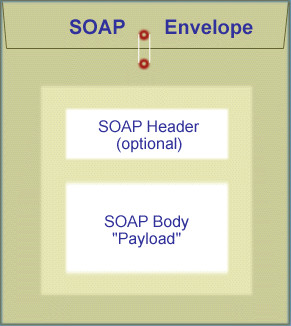
\includegraphics[scale=0.5]{soap_envelope.jpg}\\
  \caption{SOAP Envelop}
  \label{fig:soap_env}
\end{figure}

\paragraph{SOAP Message Example:}

The following example gives an overview of a SOAP message:

\lstset{language=XML}
\begin{lstlisting}
<?xml version="1.0"?>
<soap:Envelope xmlns:soap="http://www.w3.org/2003/05/soap-envelope">
  <soap:Header>
  </soap:Header>
  <soap:Body>
    <m:GetStockPrice xmlns:m="http://www.example.org/stock">
      <m:StockName>IBM</m:StockName>
    </m:GetStockPrice>
  </soap:Body>
</soap:Envelope>
\end{lstlisting}

\subsubsection{REST\label{sec:back_tech_ws_rest}}
In addition to SOAP, there is another alternative for the implementation of Web services. \citeauthor{Fielding2000} in his dissertation describes an architectural style that he calls REpresentational State Transfer architecture or short REST.

REST is based on principles that are used in the largest distributed application - the World Wide Web. The World Wide Web is itself a gigantic REST application. Many search engines, shops or booking systems have unintentionally been based on REST web services.

The REpresentational State Transfer Architecture is an architectural model, which describes how the Web should work. The model will serve as a guide and reference for future enhancements.

REST is not a product or standard. REST describes how web standards in a Web-friendly manner can be used.


\paragraph{REST Example:} An online store will serve here as an example of a RESTful application. In this application, there are customers who can place items in shopping carts.

Each object of the application, such as the product or the customer is a resource that is externally accessible via a URL. With the following request in the example application, the shopping cart with the number 7621 is retrieved.

%\lstset{language=JSON}
\begin{lstlisting}
GET /cart/7621
\end{lstlisting}

It is not specified in REST how the result of a request is represented. Client and server must have a shared understanding how the data is represented, i.e. in XML or JSON. The following example is a response in JSON format.

%\lstset{language=JSON}
\begin{lstlisting}
{
"customer": 7621,
"articles":[
	{"position":1,
	"articleNumber"=89,
	"description":"iPhone5",
	"price":200},
	{"position":2,
	"articleNumber"=76,
	"description":"Samsung Galaxy S III",
	"price":150}
]
}
\end{lstlisting}

\subsubsection{SOAP vs. REST TODO\label{sec:back_soap_vs_rest}}

The main advantages of REST web services is that they are lightweight, without a lot of extra XML markup. Also REST has easy to read results and is easy to build requiring no special tool-kits.

SOAP also has some advantages, usually it is easy to use, provides relatively strong typing since it has a fixed set of supported data types, furthermore many different kinds of development tools are available.

Next some aspects of SOAP and REST will be compared.

\paragraph{API Flexibility \& Simplicity}

The key to the REST methodology is to use an interface that is already well known and widely used, the URI, in order to write web services. For example, providing a currency converter service, in which a user types-in the desired currencies for input and output and the specific amount in order to receive a real-time conversion, could be as simple as making a script accessible on a Web server via the following URI: http://www.currencyconverter.com\/convert?in=us-dollar\&value=100\&out=euro

This service could easily be requested with an HTTP GET command by any client or server application with HTTP support. The resulting HTTP response depends on how the service provider wrote the script and it might be as simple as some standard headers and a text string containing the current price for the given currencies, or it might be an XML document.
\\
\\
The significant advantages of this interface method over SOAP-based services are as follows:-
\\
\\
The creation and modification of a URI in order to access different web resources can easily be figured out by any developer. However, in order for SOAP to be used, most developers would need a SOAP toolkit to form requests and obtain the results, as it requires specific knowledge of a new XML specification.
\\
\\
\paragraph{Bandwidth Usage}

The RESTful interface has short requests and responses, which is another advantage. Whereas, an XML wrapper around every request and response is required for SOAP. For a four- or five-digit stock quote, a SOAP response may require more than 10 times the number of bytes as the same response in REST, as SOAP requires namespaces and typing to be present. 
\\
\\
\paragraph{Security}
The security perspective debate is probably the most interesting aspect of the comparison between REST and SOAP. 

Sending remote procedure calls (RPC) through standard HTTP ports is seen by the SOAP camp as being a good way to ensure Web services support across organizational boundaries. In contrast however, REST followers see this as compromising network safety and considers this practice a major design flaw.

With REST, the administrator (or firewall) can discern the intent of each message by analyzing the HTTP command used in the request, even though the REST calls also go over HTTP or HTTPS. For example, a GET request is always seen as being safe because by definition, the data cannot be modified. It can only query data.

On the other hand, HTTP POST is used by a typical SOAP request to communicate with a given service. Without looking into the SOAP envelope, it is not possible to know whether the request simply wants to query data or delete entire tables from the database. This task is resource-consuming and it is not built into most firewalls.

On the downside with SOAP, the difficult task of authentication and authorization is left up to the application developer. However, the fact that the web servers already have support for these tasks, is taken into account by the REST methodology. REST methodology developers can make the network layer do all the heavy work by using industry-standard certificates and a common identity management system, such as an LDAP server.

However, REST is not perfect. It is not always the best solution for every web service. Data should never be sent as parameters in URIs in order to be kept secures. 

\paragraph{Type Handling}

Due to its fixed set of supported data types, SOAP provides a stronger typing. In this way, it ensures a return value  will be given in the corresponding native type in a specific platform. For example, when an API is HTTP based, the return value will need to be deserialized from its original XML format before being type-casted.    
However, handling complex data-types proves to be the main challenge and is mainly achieved by defining a serialization and deserialization mechanism, wherefore there is no definitive advantage concerning ease of client-side coding. 


\paragraph{Client-side Complexity}

Making calls to an REST API poses less of a challenge than making calls to a SOAP API. While REST is elementary to all programming languages and merely implies constructing an HTTP request with the appropriate parameters, the latter requires a client library, a Stub and involves additional learning effort.  

\paragraph{Testing and Troubleshooting}

A further characteristic of REST APIs is their easy testing and troubleshooting ability, requiring no more than a browser, the response appearing in the browser window itself. Generating a request does not require special test tools, this is a major advantage of REST based APIs.  
  

\paragraph{Server-side Complexity}

The majority of programming languages provide easy to operate mechanisms to expose a method using SOAP. However exposing a method using REST based APIs, involves additional effort due to the task of mapping the URI path to specific handlers. Though various frameworks facilitate this task, the exposition of methods is still easier to achieve using SOAP than REST.

\paragraph{Caching}

To consume a REST based API service, a simple GET request is needed, therewith allowing proxy servers to cache their response very easily. In contrast, SOAP requests use POST and require a complex XML format, producing difficulties for response-caching.

\subsection{NoSQL Databases TODO NoSQL Evaluation\label{sec:back_da_per}}
SQL databases have been used to solve storage problems for a long time, including cases in which there is a high discrepancy between the object model and its relational model. The conversion of graphs to tables represents yet another dis-functional use of data mapping. The complex structure this sort of mismanagement causes depends on mapping frameworks and complex algorithms. The rigid relational scheme characteristic for SQL becomes especially inefficient for such web applications as blogs due to their multifaceted range of attributes that need to be stored in their respective tables, e.g. comments, pictures, audios, videos, source codes. Therefore adding or removing a new feature to this sort of website will necessarily result in system unavailability.          

Nowadays of course,  web sites are developing towards more interactive models, obliging databases to perform real-time scheme updates, thereby paving the way for NoSQL to provide a database molded for modern demands. %The following section describes the characteristics of NoSQL and its different types of databases.   

%\subsubsection{SQL\label{sec:back_da_per}}
%\subsubsection{NoSQL\label{sec:back_da_per}}	

There is a variety of ideas surrounding the NoSQL movement, however the core idea is to provide more flexible data models, as opposed to the SQL approach, in order to provide live scheme updates. The ever increasing amount of data streaming through the web implies challenges, which any competitive website wishing to stay in business will have to meet. Besides dealing with vast amounts of data, these sites have to respond to constant requests around the globe without allowing any noticeable latency.

To this end, many companies have developed their own storage systems, according to their specific needs, which have been classified as NoSQL databases. Considering the fact that these stores are set up to fulfill the individualized requirements of the companies they belong to, there can be no final answer as to which of them  works most efficiently. For example, Facebook implemented the NoSQL database Cassandra in order to solve the so called "Inbox Search Problem" - the challenge of allowing Facebook users to search through their sent and received messages - caused by the multitude of stored data alongside the high number of active users. 
--------------------
\\
\\
A selection of the best known NoSQL systems are shown in Table , which are categorized into the following groups: Key Value Stores, Document Stores, Column Family Stores and  Graph Databases
\\
\\
\begin{tabular}{|c|c|c|c|}
\hline 
\textbf{Key Value Stores} & \textbf{Document Stores} & \textbf{Column Stores} & \textbf{Graph Databases} \\ 
\hline 
$\begin{array}{l} \textbf{Riak} \\ \textbf{Amazon SimpleDB} \\ \textbf{Voldemort}\\  \textbf{Redis} \end{array}$ & 
$\begin{array}{l} \textbf{CouchDB} \\ \textbf{MongoDB} \\ \textbf{Couchbase} \end{array}$ & 
$\begin{array}{l} \textbf{HBase} \\ \textbf{Hypertable} \\ \textbf{Cassandra}  \end{array}$  & 
$\begin{array}{l} \textbf{Neo4J} \\ \textbf{AllegroGraph}   \end{array}$ \\ 
\hline 
\end{tabular}
\\
\\

The following sections will examine these groups, each accompanied by one or more exemplary implementations.      

\subsubsection{Key Value Stores}

Key value stores provide suitable storage systems for simple operations, based on key attributes only. They can be compared to maps or dictionaries due to the fact that data is identified by a unique key. They allow for a user specific webpage to be partially calculated beforehand and consequently be served quickly to the user when requested. Most key value stores save their data in memory, so they are frequently used for caching of SQL queries, which result more time intensive. Examples for key value stores are Project Voldemort, Redis,Membase and Riak of which the latter will be described in detail in the following paragraph.

\paragraph{Riak:} Riak is a distributed, scalable, open source key/value store. Riak scales predictably and easily and simplifies development by giving users the ability to quickly prototype, test, and deploy their applications. One of two ways to access data in Riak by using a REST API. The other way to access data is through a fully-featured Protocol Buffers API. This is a simple binary protocol based on the library Google's open source project of the same name.

The only one way to organize data inside of Riak is by using buckets and keys. Data is stored and referenced by bucket/key pairs. These buckets are used to define a virtual keyspace and provide the ability to define isolated non-default configuration. They might be compared to tables or folders in relational databases or file systems, respectively \cite{Riak:Buckets}.

Interactions with Riak are mostly setting or retrieving the value of a key. The following describes how to do that using the Riak HTTP API. To read an object, this is a basic command formation for retrieving a specific key from a bucket. 

\begin{code}
\begin{minted}[frame=single]{console}
GET /riak/bucket/key
\end{minted}
%\caption{My Func}
\label{lst:riak_get}
\end{code}

The body of the response will contain the contents of the object (if it exists).
\\
\\
For storing an object with a user-defined key, the basic request looks like this:

\begin{code}
\begin{minted}[frame=single]{console}
PUT /riak/bucket/key
\end{minted}
%\caption{My Func}
\label{lst:riak_get}
\end{code}

There is no need to explicitly create a bucket because they are automatically created when keys added to them.


\subsubsection{Document Stores}
Document Stores interlace key value pairs in JSON or JSON like documents. Each of these documents contains a special key "ID", which is unique throughout a collection of documents and therefore identifies a document explicitly. 

Key value stores don't allow for values to be queried, because the values are only accessible through their respective keys. Document stores on the other hand provide mechanisms for this additional function. They therefore allow complex data structures to be handled more efficiently. The interpretable JSON format applied by document stores ensures a developer friendly handling by supporting data types. In contrast to key value stores which focus on high performance for read and write concurrent, document stores concentrate on storing big data efficiently while also providing a high query performance. Most known document stores are CouchDB and MongoDB  which are described in detail in the following paragraphs.

%--------------
\paragraph{CouchDB:} Apache CouchDB is a free and open-source document-oriented database written in Erlang, a programming language aimed at concurrent and distributed applications. It was firstly released in 2005 and later became an Apache project in 2008.

CouchDB implements a form of Multi-Version Concurrency Control (MVCC) in order to avoid the need to lock the database file during writes. Conflicts are left to the application to resolve. Resolving a conflict generally involves first merging data into one of the documents, then deleting the stale one.

CouchDB stores data in semi-structured documents. A document is a JSON file which is a collection of named key-value pairs. Values can either be numbers, string, booleans, lists or dictionaries. The documents are completely schema-free and do not have to follow any structure (except for JSON’s inherent structure).

An example document is shown in Listing \ref{lst:couch_doc}, which represent the apple price in various supermarket. 
\\
\\
\begin{code}
\begin{minted}[frame=single]{json}
{
    "_id" : "bc2a98726578c326ec68382f846d7629",
    "_rev" : "8763642898",
    "item" : "apple",
    "prices" : {
        "ALDI" : 1.59,
        "LIDL" : 5.99,
        "Kaufland" : 0.79
    }
}
\end{minted}
\caption{Example of a CouchDB document}
\label{lst:couch_doc}
\end{code}

Each document in a CouchDB database is identified by a unique ID (the 'id' field). CouchDB is a simple container of a collection of documents and it does not establish any mandatory relationship between them [ALS10].  CouchDB exposes a RESTful HTTP API to perform basic CRUD operations on all stored items and it uses the HTTP methods POST, GET, PUT and DELETE to do so.

As illustrated in figure \ref{fig:couchdb_repl}, one can synchronize the data between any two databases easily. After replication, each database is able to work independently.
% TODO cite http://guide.couchdb.org/draft/consistency.html
\begin{figure}[htb]
  \centering
  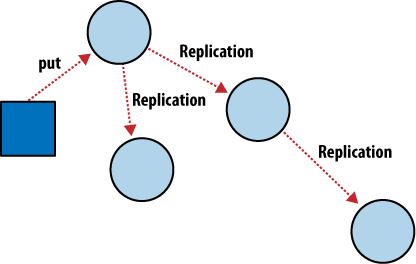
\includegraphics{couchdb_repl.png}\\
  \caption{CouchDB replication}
  \label{fig:couchdb_repl}
\end{figure}

\pagebreak
\pagebreak
For conflict handling, CouchDB relies on the MVCC model. Each document is assigned a revision id and every time a document is updated, the old version is kept and the updated version is given a different revision id. Whenever a conflict is detected, the winning version is saved as the most recent version and the losing version is also saved in the document’s history. This is done consistently throughout all the nodes so that the exact same choices are made. The application can then chose to handle the conflict by itself (ignoring one version or merging the changes) [ALS10].


\paragraph{MongoDB:\label{sec:back_mongo}}
MongoDB (from “humongous”) is a free and open-source document-oriented database written in C++ [10g11d]. Aside from the open-source community, the development is also supported by the company 10gen.
It is completely schema-free and manages JSON-style documents, as in CouchDB. It focuses on high-performance and agile development, providing the developer with a set of features to easily model and query data, as well as to scale the system.

MongoDB stores data as BSON objects, which is a binary-encoded serialization of JSON-like documents. It supports all the data types that are part of JSON but also defines new data types, i.e. the Date data type and the BinData type [BSO11]. The key advantage of using BSON is efficiency (both in space and compute time), as it is a binary format [10g09].
Documents are contained in 'collections', they can be seen as an equivalent to relational database tables [10g11b]. Collections can contain any kind of document, no relationship is enforced, still documents within a collection usually have the same structure as it provides a logical way to organize data.
As data within a collections is usually contiguous on disk, if collections are smaller better performance is achieved [10g11h]. Each document is identified by a unique ID ( 'id' field), which can be given by the user upon document creating or automatically generated by the database [10g11e]. An index is automatically created on the ID field although other indexes can be manually created in order to speed up common queries.

Two forms of replication are available, Replica Sets and Master-Slave, see figure \ref{fig:mongodb_repl}. As Master-Slave replication is deprecated since version 1.6, Replica Sets are used for all new production deployments.

% TODO cite http://guide.couchdb.org/draft/consistency.html
\begin{figure}[htb]
  \centering
  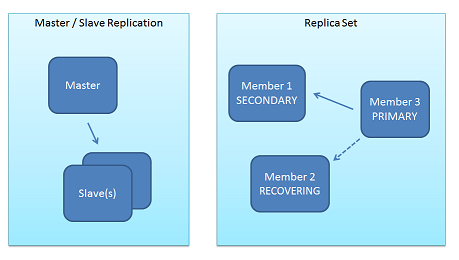
\includegraphics{mongodb_repl.png}\\
  \caption{MongoDB replication}
  \label{fig:mongodb_repl}
\end{figure}

%-----------
\subsubsection{Column Stores}
Column Family Stores are also known as column oriented stores, extensible record stores and wide columnar stores TODO cite. All stores are inspired by Googles Bigtable, which is a "distributed storage system for managing structured data that is designed to scale to a very large size" [12] TODO cite. Google has been using Bigtable in many projects with varying requirements of high throughput and latency-sensitive data serving. The data model is described as "sparse, distributed, persistent multidimensional sorted map" [12] TODO cite. In this map, an arbitrary number of key value pairs can be stored within rows. Values cannot be interpreted by the system, therefore relationships between datasets and any other data types than strings are not supported natively. These additional features have to be implemented in the application logic as is also the case when handling key value stores. In order to achieve both versioning and consistency, multiple versions of a value are stored chronologically. 

Big companies such as Google and Facebook, use their respective Column Family Stores (Big Table and Cassandra) to store data in the same way as it will eventually be required when requested. This sort of storage  ensures that only one data retrieval is needed when a request is launched, therefore saving considerable effort and maximizing performance when compared to the conventional process via MySQL which often requires multiple queries.  

%---------------
\paragraph{Cassandra}
Apache Cassandra is a free and open-source distributed, structured key-value store with eventual consistency. It is a top-level project of the Apache Foundation and it was initially developed by Facebook [Fou11h]. It is designed to handle very large amounts of data, while providing high availability and scalability.

(cite Cassandra) A table in Cassandra is a distributed multi dimensional map indexed by a key. The value is an object which is highly structured. The row key in a table is a string with no size restrictions, although typically 16 to 36 bytes long. Every operation under a single row key is atomic per replica no matter how many columns are being read or written into. Columns are grouped together into sets called column fam- ilies very much similar to what happens in the Bigtable[4] system. Cassandra exposes two kinds of columns families, Simple and Super column families. Super column families can be visualized as a column family within a column family.
Furthermore, applications can specify the sort order of columns within a Super Column or Simple Column family. The system allows columns to be sorted either by time or by name. Time sorting of columns is exploited by application like Inbox Search where the results are always displayed in time sorted order. Any column within a column family is accessed using the convention column family : column and any column within a column family that is of type super is accessed using the convention column family : super column : column. A very good example of the super column family abstraction power is explained below.

For Inbox Search we maintain a per user index of all mes- sages that have been exchanged between the sender and the recipients of the message. There are two kinds of search features that are enabled today (a) term search (b) interactions - given the name of a person return all messages that the user might have ever sent or received from that person. The schema consists of two column families. For query (a) the user id is the key and the words that make up the message become the super column. Individual message identifiers of the messages that contain the word become the columns within the super column. For query (b) again the user id is the key and the recipients id's are the super columns. For each of these super columns the individual message identifiers are the columns. In order to make the searches fast Cassandra provides certain hooks for intelligent caching of data. For instance when a user clicks into the search bar an asynchronous message is sent to the Cassandra cluster to prime the buffer cache with that user's index. This way when the actual search query is executed the search results are likely to already be in memory. The system currently stores about 50+TB of data on a 150 node cluster, which is spread out between east and west coast data centers. We show some production measured numbers for read performance.

\begin{tabular}{|c|c|c|}
\hline 
Latency Stat & Search Interactions & Term Search \\ 
\hline 
Min & 7.69ms & 7.78ms \\ 
\hline 
Median & 15.69ms & 18.27ms \\ 
\hline 
Max & 26.13ms & 44.41ms \\ 
\hline 
\end{tabular} 
%---------------

\subsubsection{Graph Databases:}
(cite NoSQL Evaluation) In contrast to relational databases and the already introduced key oriented NoSQL databases, graph databases are specialized on efficient management of heavily linked data. Therefore, applications based on data with many relationships are more suited for graph databases, since cost intensive operations like recursive joins can be replaced by efficient traversals.
Neo4j [16] and GraphDB [17] are based on directed and multi relational property graphs. Nodes and edges consist of objects with embedded key value pairs. The range of keys and values can be defined in a schema, whereby the expression of more complex constraints can be described easily. Therefore it is possible to define that a specific edge is only applicable between a certain types ofnodes.
Property graphs are distinct from resource description framework stores like Sesame [18] and Bigdata [19] which are specialized on querying and analyzing subject-predicate-object statements. Since the whole set of triples can be represented as directed multi relational graph, RDF frameworks are considered as a special form of graph databases in this paper, too. In contrast to property graphs, these RDF graphs do not offer the possibility of adding additional key value pairs to edges and nodes. On the other handy, by use of RDF schema and the web ontology language it is possible to define a more complex and more expressive schema, than property graph databases do.
Twitter stores many relationships between people in order to provide their tweet following service. These one-way relationships are handled within their own graph database FlockDB [20] which is optimized for very large adjacency lists, fast reads and writes.
Use cases for graph databases are location based services, knowledge representation and path finding problems raised in navigation systems, recommendation systems and all other use cases which involve complex relationships. Property graph databases are more suitable for large relationships over many nodes, whereas RDF is used for certain details in a graph. FlockDB is suitable for handling simple I-hop-neighbor relationships with huge scaling requirements.
\paragraph{Neo4J}
%neo4j ist eine von der Firma Neo Technology seit 2007 entwickelte, in Java im- plementierte, hochskalierende und hochverfu ̈gbare Graphendatenbank, die unter der GPL/AGPL 3.0 vero ̈ffentlicht wird.

%Relationale Datenbanken erfordern die U ̈bertragung der Knoten und Kanten eines Graphenmodells in die Form von Datenbanktabellen. Im Gegensatz dazu unterstu ̈tzt neo4j diese Graphenelemente nativ, was die Modellierung von in Graphen strukturierten Problemdom ̈anen vereinfacht. Im Folgenden seien die wichtigsten Bestandteile des neo4j Datenmodells kurz beschrieben:
%Knoten. Knoten bilden die grundlegenden Einheiten eines Graphen. Jeder Knoten ist in neo4j mit einer eindeutigen, fortlaufenden ID versehen. Knoten ko ̈nnen optional auch Eigenschaften besitzen, bei denen es sich um einfache Schlu ̈ssel/Werte-Paare handelt. Diese mu ̈ssen keinem vorgegebenen Schema fol- gen, d.h. die verwendeten Schlu ̈ssel ko ̈nnen sich von Knoten zu Knoten unter- scheiden. Dies stellt eine erhebliche Flexibilisierung im Vergleich zu relationalen Datenbanken dar, welche fu ̈r jeden Knotentyp eine eigene Tabelle erfordern wu ̈rden.
%Ein spezieller Knoten in neo4j ist der sogenannte Referenzknoten. Er existiert in jeder neu angelegten neo4j Datenbank und stellt einen allgemein bekannten Einstiegspunkt fu ̈r jeden Graphen dar[AN10]. Es wird geraten jeden Knoten zumindest indirekt mit diesem Knoten zu verbinden, so dass jeder Knoten der Datenbank vom Referenzknoten aus erreichbar ist.
%Kanten. Kanten verbinden Knoten und stellen die Auffindbarkeit derselben in der Datenbank sicher. Wie Knoten auch ko ̈nnen sie eindeutig u ̈ber eine ID iden- tifiziert werden. Zu jeder Kante geho ̈hrt zwingend ein Start- und ein Endknoten, sowie ein Typbezeichner.
%Kanten sind immer gerichtet. Die Tatsache, dass X Fan von Y ist, heißt noch lange nicht, dass Y auch Fan von X ist. Sollte die Richtung der Verbindung keine Rolle spielen, kann sie beim Traversieren des Graphen auch ignoriert werden.
%Wie Knoten auch ko ̈nnen Kanten optional schemalose Eigenschaften in Form von Schlu ̈ssel/Werte-Paaren enthalten.

%Pfade. Pfade sind die Aneinandereihung mehrerer Knoten anhand von Kanten und vor allem deshalb wichtig, weil sie h ̈aufig das Ergebnis von Suchanfragen an die Datenbank darstellen.
%Indizes. Knoten und Kanten ko ̈nnen jeweils anhand ihrer Eigenschaft indiziert werden. Suchanfragen wie ”gib’ mir alle Knoten, deren Vorname ’Bernd’ ist”, ko ̈nnen auf diese Weise wesentlich schneller abgearbeitet werden als wenn der gesamte Graph nach passenden Knoten durchsucht werden mu ̈sste.

%neo4j bietet zwei verschiedene Arten des Betriebs an (siehe Fig 1.). Zum einen kann neo4j ”embedded” betrieben werden, das heißt als Teil einer Applikation mit direktem Zugriff auf die auf der Festplatte befindliche Datenbank; zum an- deren als ein Server zu dem man sich als Client verbindet,  ̈ahnlich wie man dies von traditionellen relationalen Datenbanksystemen her gewohnt ist.
%Da der neo4j Server prinzipiell auf neo4j Embedded fußt, sei dieses im Folgenden zun ̈achst n ̈aher beschrieben.
bla bla:

\begin{figure}[htb]
  \centering
  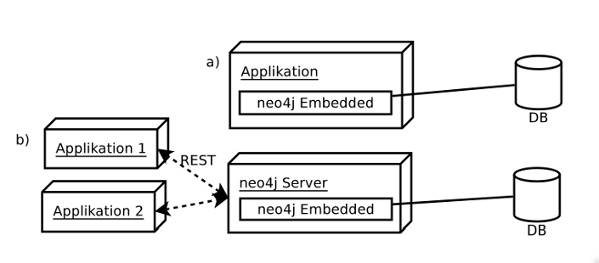
\includegraphics[scale=0.4]{neo4j.png}\\
  \caption{Embedded (a) vs. Server (b)}
  \label{fig:neo4j}
\end{figure}



\subsection{Message Queue\label{sec:back_me_mid}}
Message queues provide an asynchronous communications protocol, meaning that the sender and receiver of the message do not need to interact with the message queue at the same time. Messages placed onto the queue are stored until the recipient retrieves them. Message queues have implicit or explicit limits on the size of data that may be transmitted in a single message and the number of messages that may remain outstanding on the queue.

There are a number of open source choices of messaging middleware systems, including JBoss Messaging, JORAM, Apache ActiveMQ, Sun Open Message Queue, Apache Qpid, RabbitMQ, Beanstalk'd, Tarantool and HTTPSQS

\paragraph{RabbitMQ}

%RabbitMQ ist ein Open-Source-Message-Broker, welcher den AMQP Standard implementiert. Rabbit Technologies Ltd., die Firma hinter RabbitMQ, welche ehemals aus der Firma LShift ausgegründet wurde, ist im April 2010 von SpringSource, einem VMWare Unternehmen, übernommen worden.[41]
%In RabbitMQ und dessen Nachrichtenmodell gibt es vier grundlegende Komponenten. Diese sind in der Abbildung 2.4 zu sehen. Einen Produzenten (P) und Konsumenten (C), eine Message-Queue (Q) und einen Exchange (X). Der Produzent ist ein Programm, welches Nachrichten versendet, die in einem Pu􏰊er, der Message-Queue, abgelegt werden und solange darin verbleiben, bis ein Konsument diese aus dem Pu􏰊er wieder entnimmt.
bla bal TODO cite fig http://www.rabbitmq.com/tutorials/amqp-concepts.html
\begin{figure}[htb]
  \centering
  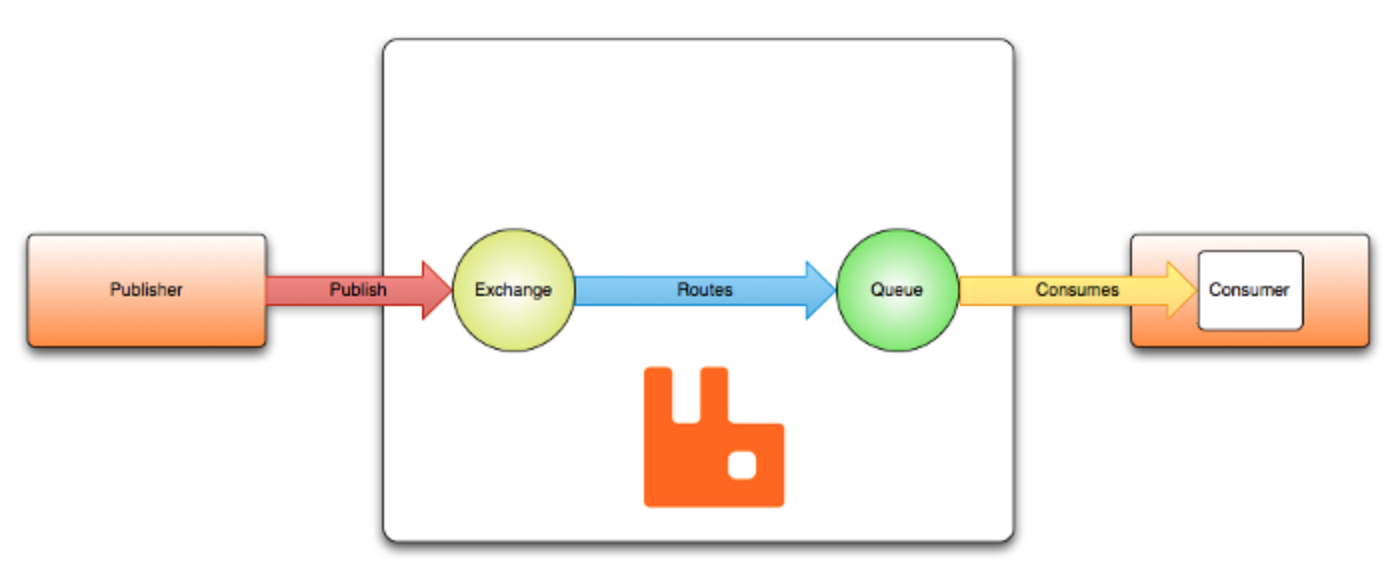
\includegraphics[scale=0.6]{rabbit_mq.png}\\
  \caption{RabbitMQ Components}
  \label{fig:rabbit_mq}
\end{figure}

%Der Produzent schickt dabei eine Nachricht niemals direkt in eine Message-Queue, sondern an einen Exchange. Diese einfache Komponente empfängt die Nachrichten von dem Produzenten und leitet diese an Message-Queues weiter. Dabei muss der Exchange genau wissen, was er mit den empfangenen Nachrichten machen soll. Hierfür gibt es Regeln, welche von vier verschiedenen Exchange-Typen definiert sind: direct, topic, headers und fanout.

Direct exchange witer vom http://www.rabbitmq.com/tutorials/amqp-concepts.html
bla bal TODO cite fig http://www.rabbitmq.com/tutorials/amqp-concepts.html
\begin{figure}[htb]
  \centering
  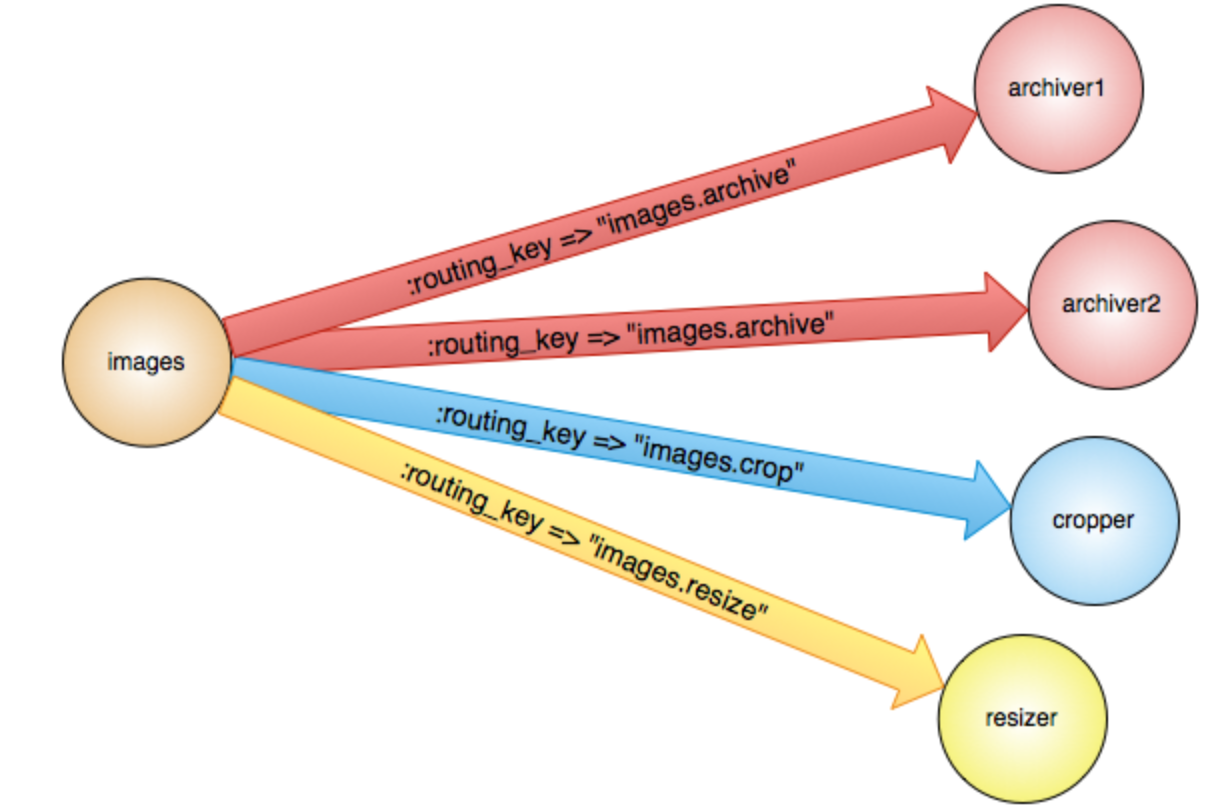
\includegraphics[scale=0.6]{rabbit_mq_direct.png}\\
  \caption{Direct exchange routing}
  \label{fig:rabbit_mq_direct}
\end{figure}


%Der fanout-Exchange leitet immer alle empfangenen Nachrichten an alle verbundenen Message-Queues weiter. Bei den restlichen Typen erfolgt eine Weiterleitung ausschließlich an Message-Queues, die ein bestimmtes Kriterium erfüllen. Diese Kriterrien werden beim Verbinden der Message-Queues mit den Exchanges mittels eines Bindingkeys angegeben. Erreicht nun eine Nachricht einen Exchange, überprüft dieser, ob der Routing-Key in der Nachricht mit dem Binding-Key der Queue übereinstimmt. Ist dies der Fall, wird diese Nachricht an die jeweilige Queue geleitet. Andernfalls wird die Nachricht verworfen [45].
bla bal TODO cite fig http://www.rabbitmq.com/tutorials/amqp-concepts.html
\begin{figure}[htb]
  \centering
  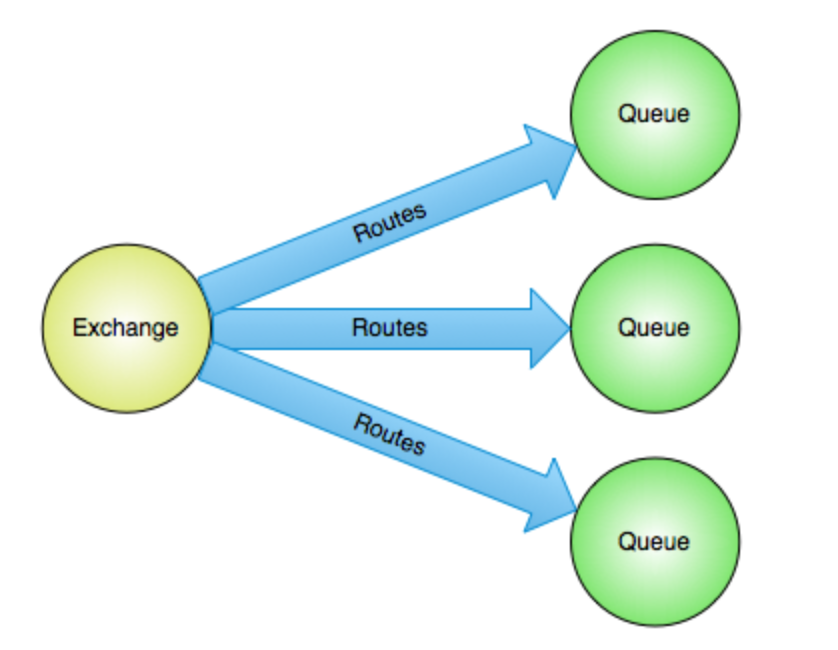
\includegraphics[scale=0.6]{rabbit_mq_fanout.png}\\
  \caption{Fanout exchange routing}
  \label{fig:rabbit_mq_fanout}
\end{figure}

\paragraph{ActiveMQ}
%Ebenso wie bei RabbitMQ aus dem vorherigen Absatz handelt es sich bei Apache ActiveMQ um einen Message Broker. Dieser ist jedoch in Java geschrieben und im- plementiert nicht das AMQP Protokoll, sondern das Java Message Service (JMS) Protokoll in der Version 1.1 vom 12.04.2002. Der Vorteil gegenüber RabbitMQ ist, dass sich dieser Broker in eine Java-Anwendung einbetten lässt und das Ausliefern eines Softwarepaketes somit vereinfacht.
%In der Abbildung 2.5 sind die verschiedenen Komponenten des Java Message Ser- vive und deren Beziehungen zueinander abgebildet. Java Message Service bietet zwei Nachrichtenmodelle an. Zum einen das Point-to-Point-Modell und zum anderen das Publish/Subscribe-Modell an. [35]
%Bei dem Point-to-Point-Modell besitzt jede Nachricht genau einen Empfänger, der den Erhalt einer Nachricht dem Sender quittiert. Dabei werden gesendete Nachrich- ten in einer Warteschlange abgelegt und verbleiben darin bis der Empfänger diese aus der Warteschlange entnimmt.
%Anders verhält es sich bei dem Publish/Subscribe-Modell. Hier kann eine Nach- richt gleich mehrere Empfänger besitzen, je nachdem wie viele Klienten ein Topic abonniert haben. Gesendete Nachrichten werden nicht in einer Warteschlange zwi- schengespeichert, sondern sofort an alle Abonnenten geschickt, d.h. es können erst Nachrichten zu einem Thema empfangen werden, nachdem ein Abonnement für ein Topic vereinbart wurde. Der Abonnent muss jedoch die ganze Zeit für das Empfangen von Nachrichten bereit sein.
\subsection{Search Platforms \label{sec:back_se_en}}
Search engines are designed to help users to quickly find useful information from the web. Thousands number of search engines are existing to perform the task of information retrieval but only some of them are popular. Because of vast availability of numerous search engines searchers often get confuse with the problem of good search engine selection.

User queries are becoming more complex and personalized over time, and much of the data required to deliver an appropriate response is inherently unstructured. Where once an SQL LIKE clause was good enough, today's usage sometimes calls for sophisticated algorithms. Fortunately, a number of open source and commercial platforms address the need for pluggable search technology, including Lucene, Sphinx, Solr, Amazon's CloudSearch, and Elasticsearch.
\subsubsection{Apache Solr \label{sec:back_se_solr}}
cite https://svn.apache.org/repos/asf/lucene/dev/branches/lucene3622/solr/site/index.pdf

Solr is the popular, blazing fast open source enterprise search platform from the Apache Lucene project. Its major features include powerful full-text search, hit highlighting, faceted search, dynamic clustering, database integration, rich document (e.g., Word, PDF) handling, and geospatial search. Solr is highly scalable, providing distributed search and index replication, and it powers the search and navigation features of many of the world's largest internet sites.
Solr is written in Java and runs as a standalone full-text search server within a servlet container such as Tomcat. Solr uses the Lucene Java search library at its core for full-text indexing and search, and has REST-like HTTP/XML and JSON APIs that make it easy to use from virtually any programming language. Solr's powerful external configuration allows it to be tailored to almost any type of application without Java coding, and it has an extensive plugin architecture when more advanced customization is required.

\subsubsection{Elasticsearch \label{sec:back_se_es}}
cite CERN:

Elasticsearch provides both an indexing service as well as a data store. It does not require a
detailed schema , although one may be provided if needed. Any data that we can express as
JSON can be easily stored and indexed with Elasticsearch.

Since elasticsearch is schema-less unless explicitly defined, any JSON documents can be added to elasticsearch, see following example:
 
\begin{code}
\begin{minted}[frame=single]{console}
curl -XPUT http://localhost:9200/blogs/blog/1 -d '{
    "post_date": "2012-12-15T09:00:00",
    "content": "This is the first blog"
}'

curl -XPUT http://localhost:9200/blogs/blog/2 -d '{
    "author": "abdul",
    "post_date": "2012-12-16T11:00:00",
    "content": "Second blog"
}'
\end{minted}
\caption{schema free elasticsearch}
\label{lst:elasticsearch_schema-free}
\end{code}
Internally, elasticsearch uses a NoSQL database system supporting JSON documents. Due to multi
tenancy, an elasticsearch instance can have more than one index. An index consists of types which
consist of fields. In accordance to relational database systems, an index is equivalent to a database, a
type is comparable to a table and a field is comparable to a column. No type schema definition is
necessary which makes elasticsearch highly flexible. Indexes and types are created automatically if
they do not exist yet. Types such as numbers and dates are automatically detected and treated accordingly.

Elasticsearch offers so-called 'multi tenancy' allowing documents to be divided into seperate 'indexes'. An index is equivalent to a database in relational database systems. Elasticsarch offers 'sharding' allowing indexes to be broken up into smaller 'shards'. 
Replication for indexes and shards allows a distributed environment with copies on different nodes. Another design goal of elasticsearch is near real-time search also supported in multi tenant and multi node environments.


One of the unique features of Elasticsearch that makes it especially well suited for our purposes is the ease with which we can scale our solution. It provides us with the ability to either
add or remove resources (that is, individual machines running Elasticsearch) at any time. We
might do this in order to support a growing data set or, perhaps, in order to satisfy an increasing amount of requests and to improve the performance of our solution.

%\subsection{Web Servers\label{sec:back_we_se}}
%bla
%\subsubsection{Apache \label{sec:back_ap}}
%bla
%\subsubsection{NginX\label{sec:back_ng}}
%bla

\subsection{Spring Framework\label{sec:back_sp_fr}}
cite: http://static.springsource.org/spring/docs/3.2.x/spring-framework-reference/pdf/spring-framework-reference.pdf
The Spring Framework is a lightweight solution and a potential one-stop-shop for building your
enterprise-ready applications. However, Spring is modular, allowing you to use only those parts that
you need, without having to bring in the rest. You can use the IoC container, with Struts on top, but you
can also use only the Hibernate integration code or the JDBC abstraction layer. The Spring Framework
supports declarative transaction management, remote access to your logic through RMI or web services,
and various options for persisting your data. It offers a full-featured MVC framework, and enables you
to integrate AOP transparently into your software.
Spring is designed to be non-intrusive, meaning that your domain logic code generally has no
dependencies on the framework itself. In your integration layer (such as the data access layer), some
dependencies on the data access technology and the Spring libraries will exist. However, it should be
easy to isolate these dependencies from the rest of your code base.
\subsubsection{Modules}
The Spring Framework consists of features organized into about 20 modules. These modules are
grouped into Core Container, Data Access/Integration, Web, AOP (Aspect Oriented Programming),
Instrumentation, and Test, as shown in the following diagram.

%cite http://www.tutorialspoint.com/images/spring_architecture.png
%http://www.tutorialspoint.com/spring/spring_architecture.htm

\begin{figure}[htb]
  \centering
  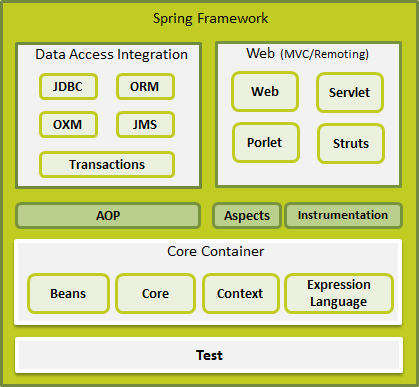
\includegraphics[scale=0.6]{spring_architecture.png}\\
  \caption{Overview of the Spring Framework}
  \label{fig:spring_arch}
\end{figure}



\paragraph{Core Container:}

The Core Container consists of the Core, Beans, Context, and Expression Language modules.

The Core and Beans modules provide the fundamental parts of the framework, including the IoC and
Dependency Injection features. The BeanFactory is a sophisticated implementation of the factory
pattern. It removes the need for programmatic singletons and allows you to decouple the configuration
and specification of dependencies from your actual program logic.

The Context module builds on the solid base provided by the Core and Beans modules: it is a means
to access objects in a framework-style manner that is similar to a JNDI registry. The Context module
inherits its features from the Beans module and adds support for internationalization (using, for example,
resource bundles), event-propagation, resource-loading, and the transparent creation of contexts by,
for example, a servlet container. The Context module also supports Java EE features such as EJB,
JMX ,and basic remoting. The ApplicationContext interface is the focal point of the Context module.

The Expression Language module provides a powerful expression language for querying and
manipulating an object graph at runtime. It is an extension of the unified expression language (unified
EL) as specified in the JSP 2.1 specification. The language supports setting and getting property values,
property assignment, method invocation, accessing the context of arrays, collections and indexers,
logical and arithmetic operators, named variables, and retrieval of objects by name from Spring's IoC
container. It also supports list projection and selection as well as common list aggregations.

\paragraph{Data Access/Integration:}
The Data Access/Integration layer consists of the JDBC, ORM, OXM, JMS and Transaction modules.

\paragraph{Web:} The Web layer consists of the Web, Web-Servlet, Web-Struts, and Web-Portlet modules.

\paragraph{AOP and Instrumentation:} Spring's AOP module provides an AOP Alliance-compliant aspect-oriented programming
implementation allowing you to define, for example, method-interceptors and pointcuts to cleanly
decouple code that implements functionality that should be separated. 

The separate Aspects module provides integration with AspectJ.

The Instrumentation module provides class instrumentation support and classloader implementations
to be used in certain application servers.

\paragraph{Test:} The Test module supports the testing of Spring components with JUnit or TestNG. It provides consistent
loading of Spring ApplicationContexts and caching of those contexts. It also provides mock objects that
you can use to test your code in isolation.

%\subsection{Application Servers\label{sec:back_sp_fr}}



\section{Related Work\label{sec:back_rel_work}}